\section{Theoretischer Hintergrund}

In diesem Kapitel sollen die wichtigsten theoretischen Grundlagen für die softwaregestützten Analyse des Einflusses der zunehmenden Netzintegration von Elektrofahrzeugen auf die Verteilnetze dargestellt und erläutert werden.
Hierzu zählen die Definition von grundlegenden Begriffen im Bezug auf Stromnetze und Elektromobilität, sowie die Vorstellung der verwendeten Softwarelandschaft mitsamt den wichtigsten Algorithmen.


\subsection{Stromnetz}

Das Stromnetz dient der Übertragung und Verteilung von elektrischer Energie. \cite{Paschotta2020}
Dabei lässt sich das Stromnetz in verschiedene Netzebenen aufteilen, welche jeweils typische Charakteristika aufweisen.
Innerhalb dieses Kapitels sollen diese kurz beschrieben werden und weitere wichtige Begriffe im Zusammenhang mit Stromnetzen erläutert werden.


\paragraph{Netzebenen:}

Das Stromnetz lässt sich grundsätzlich in Übertragungs- und Verteilnetze unterteilen.
Das Übertragungsnetz dient dem Transport von Strom über lange Strecken bei hohen Spannungen.
Ergänzend erfolgt in den Verteilnetzen die regionale Feinverteilung bei geringeren Spannungen. \cite{Agora2019}\medskip

Innerhalb der Verteilnetze wird zwischen drei Spannungsebenen unterschieden. Hierzu zählen die \glspl{HS}-, \glspl{MS}- und \glspl{NS}-Ebene.
In \autoref{tab:Spannungsebenen} finden sich die üblichen Spannungen je Spannungsebene und die verbaute Stromkreislänge in Deutschland je Spannungsebene.
Innerhalb dieser Masterarbeit werden ausschließlich die Effekte auf die Verteilnetze auf der \glspl{MS}- und \glspl{NS}-Ebene untersucht.
Zusätzlich erfolgt eine Betrachtung der Effekte auf die Umspannebene der \gls{MS}-\gls{NS}-Umspannwerke.

{
\renewcommand{\arraystretch}{1.2}% grßerer Zeilenabstand
\sisetup{range-phrase=~bis~}
\begin{table}[H]
	\begin{center}
		\caption{Übliche Spannung und Stromkreislänge der Spannungsebenen im deutschen Verteilnetz}
		\begin{tabu} to 0.65\textwidth {X[0.75] X[1, r] X[1, r]}
			\toprule
            Spannungsebene & Spannung               	& Stromkreislänge   \\\midrule
            Hochspannung   & \SIrange{60}{110}{\kv}     & \SI{95000}{\km}   \\
            Mittelspannung & \SIrange{6}{30}{\kv}  		& \SI{510000}{\km}  \\
            Niederspannung & \SI{230}{\V} 				& \SI{1100000}{\km} \\\bottomrule
            \multicolumn{3}{l}{Quellen: \cite{BDEW2016} und \cite{BMWiNetz}}
		\end{tabu}
		\label{tab:Spannungsebenen}
	\end{center}
	\vspace{-3mm}%Put here to reduce too much white space after your table
\end{table}
}


\paragraph{Netztopologie:}

\gls{NS}-Netze werden in dieser Arbeit ausschließlich als Strahlennetze ausgelegt.
Strahlennetze werden so genannt, weil die einzelnen Stränge der Netze strahlenförmig vom Ortsnetztransformator zu den Endverbrauchern verlaufen. \cite{Agora2019}
Vorteil dieser Form von Netzen ist die leichte Berechenbarkeit und die einfache Überwachung des Netzzustandes.
Jedoch führt bereits ein einziger Fehlerfall an einer Einspeisestelle eines Verbrauchers dazu, dass das auch alle nachfolgenden Verbraucher vom Netz getrennt sind.
Auch nimmt der Spannungsabfall über die Länge der Leitung immer weiter zu, was zu einer geringeren Belastbarkeit am Ende der Leitung führt. \cite{WNG2020}\medskip

Im Gegensatz dazu werden \gls{MS}-Netze als Ringnetze betrieben.
Ringnetze bieten den Vorteil, dass diese von zwei Seiten gespeist werden, wodurch ein Ringform entsteht.
Hierdurch können im Falle einer Störung weiterhin alle anderen Verbraucher versorgt werden.
Jedoch werden diese Ringnetze in der Regel offen betrieben.
Dies bedeutet, dass sich etwa in der Mitte des Rings eine offene Trennstelle befindet.
Auf diese Weise können Ringnetze ebenso einfach überwacht werden wie Strahlennetze.
Im Fehlerfall wird bei dieser Baumform maximal ungefähr die Hälfte der Verbraucher vom Netz getrennt.
Durch das Schließen der Trennstelle können dann wieder alle Verbraucher, mit Ausnahme des Fehlerfalls, versorgt werden. \cite{WNG2020} \cite{Westermann2019}


\paragraph{Gleichzeitigkeit:}

Die Gleichzeitigkeit beschreibt den Anteil der momentan anfallenden elektrischen Leistung im Bezugsgebiet von der maximalen elektrischen Leistung im Netzgebiet. \cite{Agora2019} 
Im Rahmen dieser Masterarbeit beschreibt die Gleichzeitigeit in der Regel den Anteil der momentanen elektrischen Last von \glspl{EV} im Bezug auf die installierte Leistung von Ladepunkten in einem Netzgebiet.
Ausnahmen sind entsprechend gekennzeichnet.


\paragraph{Elektrische Flexibilität:}

Elektrische Flexibilität beschreibt die Fähigkeit des Stromsystems, trotz einer vorhergesehene oder unvorhergesehene Änderungen im Verbrauch oder der Erzeugung einen Ausgleich zwischen Angebot und Nachfrage aufrecht zu erhalten.
Dabei wird die Reaktion des Stromsystems durch ein externes Signal ausgelöst.
Bei dem externen Signal kann es sich beispielsweise um ein Preissignal, aber auch ein physikalisch messbares Signal, wie die Netzfrequenz, handeln. \medskip

Elektrische Flexibilität besitzt sowohl eine zeitliche als auch eine geografische Dimension.
Die zeitliche Dimension beschreibt die zeitliche Verschiebung von Last oder Erzeugung und reicht von einer sekündlichen hin zu einer saisonalen Verschiebung.
Unter der geografischen Dimension wird die gemeinsame Nutzung von räumlich verteilten Ressourcen verstanden.
Dabei reicht die räumliche Skala von lokalen Quartierslösungen hin zu internationalen Verbundnetzen. \cite{BNetzA2017} \cite{IEA2014}


\paragraph{Residuallast:}

Die Residuallast beschreibt beschreibt die Differenz zwischen der benötigten Leistung innerhalb eines Betrachtungsgebietes und der erbrachten Leistung von nicht steuerbaren Kraftwerken.
Aufgrund des zunehmenden Anteils von nicht steuerbaren regenerativen Kraftwerken im Stromnetz und der fortschreitenden Sektorkopplung steigt zunehmend die Spreizung zwischen dem maximalen Wert und dem minimalen Wert der Residuallast.
Diese Entwicklung ist in {\color{red} TODO} dargestellt.

{\color{red} TODO: Darstellung}

Positive Residuallast wird derzeit zu großen Teilen durch regelbare Kraftwerke gedeckt, während negative Residuallast durch die Abregelung von nicht steuerbaren Kraftwerken ausgeglichen wird.
Alternativ kann eine Glättung der Residuallast auch durch die Steuerung des Verbrauches erreicht werden und vor allem negative Residuallast verhindert werden.
Hierfür bieten Elektrofahrzeuge aufgrund der hohen Ladeleistungen ein großes Potential. \cite{Paschotta2020a}


\paragraph{Netzprobleme:}

Bei der Ermittlung von Netzproblemen müssen grundlegend zwei Fälle unterschieden werden.
Im Lastfall überwiegt der Energiebedarf der Verbraucher gegenüber der Energiebereitstellung der Erzeugerkapazitäten im Netzgebiet.
Das Netz muss in diesem Fall in der Lage sein, bereitgestellte Energie aus den überlagerten Netzebenen an die Verbraucher weiterzuleiten.
Im Rückspeisefall überwiegt hingegen die Energiebereitstellung der Erzeugerkapazitäten gegenüber dem Energiebedarf der Verbraucher und der erzeugte Strom muss an die überlagerten Netzebenen weitergeleitet werden können. \cite{Agora2019}
Für die Betriebsmittel gelten die in \autoref{tab:Belastungsfaktoren} und \autoref{tab:Spannungsband} zulässigen Belastungsfaktoren und Spannungsabweichungen, welche aus \cite{Mueller2019a} entnommen wurden und auf der Verteilnetzstudie für das Land Baden-Württemberg \cite{Rehtanz2017} basieren.


\subparagraph{Verletzungen der thermische Betriebsmittelbelastungen} treten auf, wenn die physikalischen Grenzen von Betriebsmitteln bezüglich ihrer Scheinleistungsbelastung übertreten werden.
Der Belastungsfaktor eines Betriebsmittels gibt an, inwieweit ein Betriebsmittel mit Nennscheinleistung belastet werden kann.
Dabei spiegeln die Belastungsfaktoren wieder, dass für Verbraucher, welche im \gls{MS}-Netz angeschlossen sind, das (n-1)-Kriterium  gilt.
Dies gilt in der Regel jedoch nicht für Verbraucher im \gls{NS}-Netz und Erzeugerkapazitäten, welche im \gls{MS}- oder \gls{NS}-Netz angeschlossen sind.
Die Belastungsfaktoren der einzelnen Betriebsmittel sind in \autoref{tab:Belastungsfaktoren} zusammengefasst. \cite{Schachler} \cite{Rehtanz2017}


{
\renewcommand{\arraystretch}{1.2}% grßerer Zeilenabstand
\sisetup{range-phrase=~bis~}
\begin{table}[H]
	\begin{center}
		\caption{Zulässige Belastungsfaktoren der Betriebsmittel in der MS- und NS-Ebene}
		\begin{tabu} to 0.6\textwidth {X[1.6] X[0.8, r] X[1, r]}
			\toprule
			Betriebsmittel      & Lastfall           & Rückspeisefall     \\ \midrule
			MS Kabel            & \SI{50}{\percent}  & \SI{100}{\percent} \\
			NS Kabel            & \SI{100}{\percent} & \SI{100}{\percent} \\
			HS-MS-Transformator & \SI{50}{\percent}  & \SI{100}{\percent} \\
			MS-NS-Transformator & \SI{100}{\percent} & \SI{100}{\percent} \\ \bottomrule
            \multicolumn{3}{l}{Quelle: \cite{Rehtanz2017}}
		\end{tabu}
		\label{tab:Belastungsfaktoren}
	\end{center}
	\vspace{-3mm}%Put here to reduce too much white space after your table
\end{table}
}


\subparagraph{Verletzungen des Spannungsbandes} treten bei einer starken Abweichung der Spannung am Betriebsmittel von der Nennspannung auf.
Die zulässigen Spannungsabweichungen liegen für Endkunden in der \gls{NS} bei \SI{\pm 10}{\percent} und wird nach \autoref{tab:Spannungsband} auf die \gls{MS}, \gls{MS}-\gls{NS}- und \gls{NS}-Ebene aufgeteilt.
Dabei spiegelt das in der \gls{NS}-Ebene größere zulässige Spannungsband im Lastfall wieder, dass in dieser die Mehrheit der Verbraucher angeschlossen ist.
Demgegenüber wird im Rückspeisefall ein größeres Spannungsband für die \gls{MS}-Ebene reserviert. \cite{Schachler} \cite{Rehtanz2017}

{
\renewcommand{\arraystretch}{1.2}% grßerer Zeilenabstand
\sisetup{range-phrase=~bis~}
\begin{table}[H]
	\begin{center}
		\caption{Zulässige Spannungsabweichungen der Betriebsmittel in der Mittel- und Niederspannung}
		\begin{tabu} to 0.5\textwidth {X[1.2] X[1, r] X[1, r]}
			\toprule
			Spannungsebene & Lastfall               & Rückspeisefall             \\ \midrule
			MS             & \SI{-1.5}{\percent}    & \SI[retain-explicit-plus]{+5.0}{\percent}   	 \\
			MS-NS          & \SI{-2.0}{\percent}    & \SI[retain-explicit-plus]{+1.5}{\percent}   	 \\
			NS             & \SI{-6.5}{\percent}    & \SI[retain-explicit-plus]{+3.5}{\percent}   	 \\ \bottomrule
            \multicolumn{3}{l}{Quelle: \cite{Rehtanz2017}}
		\end{tabu}
		\label{tab:Spannungsband}
	\end{center}
	\vspace{-3mm}%Put here to reduce too much white space after your table
\end{table}
}


\subsection{Elektromobilität}

Innerhalb dieses Kapitels werden die für diese Masterarbeit wichtigsten Begriffe im Bezug auf die Elektromobilität erläutert und definiert.
Innerhalb dieser Arbeit werden ausschließlich die Auswirkungen der Netzintegration von \gls{EPKW} untersucht.
Der Einfluss der sonstigen Bereiche der Elektromobilität ist nicht Teil dieser Arbeit.


\paragraph{Ladetechnik:}

Die Ladetechnik von \glspl{EV} und den korrespondierenden Ladepunkten lässt sich anhand verschiedener Kriterien klassifizieren.
Innerhalb dieser Arbeit wird die Ladetechnik ausschließlich anhand der Höhe ihrer Wirkleistung unterschieden.
In \autoref{fig:four-quadrant}, finden sich die möglichen Betriebszustände der Ladetechnik von \glspl{EV} in Abhängigkeit von ihrer \gls{P} und ihrer \gls{Q}.

\begin{figure}[H]
    \centering
    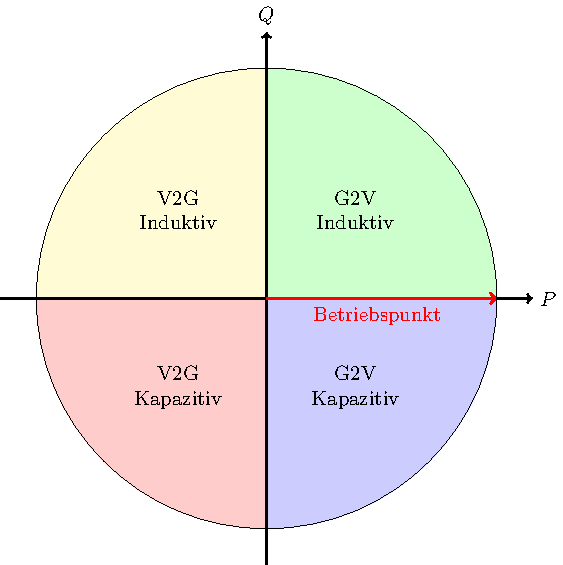
\includegraphics[width=0.7\textwidth]{Bilder/four-quadrant_operation}
    \caption{Mögliche Betriebszustände der Ladetechnik von Elektrofahrzeugen \cite{He2020}}\label{fig:four-quadrant}
\end{figure}

So können Ladevorgänge sowohl blindleistungfrei erfolgen, als auch induktiv oder kapazitiv und werden unter der Bezeichnung \gls{G2V} zusammengefasst.
In \autoref{fig:four-quadrant} entspricht dieser Modus einer positiven Wirkleistung.
Weiterhin können mit bidirektionaler Ladetechnik \glspl{EV} ebenfalls entladen werden, um beispielsweise Systemdienstleistungen zu erbringen.
Ein solcher Modus wird allgemein unter der Bezeichnung \gls{V2G} zusammengefasst und kann ebenfalls blindleistungsfrei, induktiv oder kapazitiv erfolgen.
In \autoref{fig:four-quadrant} entspricht dieser Modus einer negativen Wirkleistung. \cite{He2020} 
Innerhalb dieser Arbeit erfolgen Ladevorgänge immer blindleistungsfrei, welches dem Betriebspunkt in \autoref{fig:four-quadrant} entspricht.
Ebenfalls wird der Einsatz von bidirektionaler Ladetechnik nicht untersucht.\medskip

Die einzelnen Ladevorgänge werden anhand ihrer Wirkleistung grob in Normal- und Schnellladevorgänge unterteilt.
Normalladevorgänge finden bei einer Wirkleistung von maximal \SI{50}{\kw} statt, während Schnellladevorgänge bei einer Leistung von \SIrange[range-phrase=~{oder}~]{150}{350}{\kw} stattfinden.
Dabei besitzen die Ladevorgänge pauschal einen Wirkungsgrad von \SI{90}{\percent}.
Eine Übersicht der in dieser Arbeit verwendeten netz- und fahrzeugseitigen Wirkleistungen von Ladepunkten findet sich in \autoref{tab:charging_cap}.
Weiterhin sind die in \autoref{tab:TechPowerCap} Limitierungen der \glspl{EV} zu berücksichtigen.
Unabhängig von der Ladetechnik wird angenommen, dass am Netzverknüpfungspunkt immer einer symmetrische dreiphasige Last anliegt.

{
\renewcommand{\arraystretch}{1.2}% grßerer Zeilenabstand
\sisetup{range-phrase=~bis~}
\begin{table}[H]
	\begin{center}
		\caption{Netz- und fahrzeugseitige Wirkleistung der Ladeinfrastruktur}
		\begin{tabu} to \textwidth {X[0.5] X[1, r] X[1, r]}
			\hline
			\multicolumn{1}{l}{}           		& Netzseitige Wirkleistung & Fahrzeugseitige Wirkleistung \\ \hline
			\multirow[t]{4}{*}{Normalladung} 	& \SI{3.7}{\kw}            & \SI{3.3}{\kw}                \\
										   		& \SI{11.0}{\kw}           & \SI{9.9}{\kw}                \\
										   		& \SI{22.0}{\kw}           & \SI{19.8}{\kw}               \\
										   		& \SI{50.0}{\kw}           & \SI{45.0}{\kw}               \\ \hline
			\multirow[t]{2}{*}{Schnellladung} 	& \SI{150.0}{\kw}          & \SI{135.0}{\kw}              \\
										   		& \SI{350.0}{\kw}          & \SI{315.0}{\kw}              \\ \hline
		\end{tabu}
		\label{tab:charging_cap}
	\end{center}
	\vspace{-3mm}%Put here to reduce too much white space after your table
\end{table}
}


\paragraph{Ladestrategien:}

Der Ladevorgang von \glspl{EV} kann durch unterschiedliche äußere Anreize gesteuert werden. Grundsätzlich lassen sich hierbei marktorientierte und netzdienliche Ladestrategien unterscheiden.


\subparagraph{Marktorientierte Ladestrategien} haben als Fokus die Minimierung der Kosten für den Strombezug. Dies bedeutet konkret, dass die Ladevorgänge durch ein Preissignal am überregionalen Großhandelsmarkt ausgelöst beziehungsweise unterbrochen werden. Eine solche Ladestrategie kann sowohl positive als auch negative Effekte auf das Stromnetz aufweisen und erfordert einen geeigneten rechtlichen Rahmen. So führt beispielsweise ein hohes Stromangebot zu niedrigen Großhandelsmarktpreisen, wodurch das beladen der \glspl{EV} ausgelöst wird und ein Ausgleich zwischen Angebot und Nachfrage angestrebt wird. Auf der anderen Seite werden lokale Netzengpässe nicht berücksichtigt und die Gleichzeitigkeit der Ladevorgänge erhöht sich, wodurch sich der lokale Netzausbaubedarf erhöhen kann. \cite{Agora2019} \cite{Dorendorf2019} \cite{Rehtanz2017}


\subparagraph{Netzdienliche Ladestrategien} setzen hingegen auf die Vermeidung von lokalen Engpässen, welche durch eine hohe Nachfrage entstehen können. Hierbei kann zwischen präventiven und kurative Maßnahmen unterschieden werden. Präventive Maßnahmen sollen Kunden dazu bewegen, ihre Ladevorgänge in Zeiten geringer Netzauslastung zu verlegen. Dies kann zum Beispiel über monetäre Anreize aber auch über Quoten erfolgen. Bei kurativen Maßnahmen handelt es sich hingegen um ein aktives Eingreifen durch den Netzbetreiber, welcher bei drohenden Netzengpässen in den Ladevorgang eingreift. \cite{Agora2019}


\subsection{ding0}\label{chap:dingo_theo}

Eine der Grundlagen für die Nutzung des Netzplanungsinstruments \edisgodot, sind die zu untersuchenden Netztopologien der \gls{MS}- und \gls{NS}-Ebene.
Aufgrund der mangelnden Datenlagen von reale Netztopologien werden, wird auf synthetisch erzeugte Netztopologien zurückgegriffen.
die mit Hilfe des Open Source Tools \dingo erzeugt wurden.
Das Tool ist in der Lage ländliche und suburbane Netzstrukturen zu synthetisieren und kann auf GitHub \cite{dingo2019} öffentlich eingesehen und frei verwendet werden.
Weiterhin findet sich auf Read the Docs \cite{dingo-docs2019} eine ausführliche Dokumentation.\medskip

Die Synthetisierung der Netztopologien ist nicht Teil dieser Masterarbeit und erfolgte innerhalb des \openego Projektes. \cite{Mueller2019}
Die Netztopologien werden auf der Datengrundlage des Jahres \num{2015} gebildet und entsprechend ausgebaut.
Urbane Netzgebiete können derzeit nicht durch \dingo abgebildet werden und werden deshalb innerhalb dieser Masterarbeit nicht betrachtet.


\paragraph{Mittelspannung}

Auf der \gls{MS}-Ebene gibt es \num{3591} Netzgebiete mit einer mittleren Fläche von \SI{99}{\km\squared}.
Die einzelnen \gls{MS}-Netze werden alle als offene Ringnetze betrieben.
Im städtischen Bereich werden hauptsächlich Erdkabel mit einer Nennspannung von \SI{10}{\kv} eingesetzt, während im ländlichen Raum größtenteils Freileitungen mit einer Nennspannung von \SI{20}{\kv} eingesetzt werden. \cite{Mueller2019}\medskip

% TODO: Grafik elia study

{\color{red} TODO} zeigt den Aufbau eines beispielhaften Mittelspannungsnetzes, welches mit Hilfe von \dingo erzeugt wurde.
Die Modellierung der Mittelspannungstopologie erfolgt als Tourenplanungsproblem (Capacitated Vehicle Routing
Problem (CVRP)) in Kombination mit der Beachtung der historischen lastorientierten Entwicklung und den Planungsprinzipien von Verteilnetzen.
Ein besondere Fokus liegt dabei auf der Beachtung von Leitungsüberlastungen und Verletzungen des Spannungsbandes.
Eine genau Beschreibung der Methodik findet sich in \cite{Amme2018}.


\paragraph{Niederspannung}

Die \gls{NS}-Ebene wird mit Hilfe von \num{46} Referenznetzsträngen synthetisiert und als Strahlennetze betrieben.
Die Referenznetzsträngen stehen repräsentativ für eine bestimmte Anzahl an Hausanschlüssen und werden jeweils einer Netzklasse zugeordnet.
Hierbei wird auf Grundlage der Anzahl an Hausanschlüssen je Ortsnetzstation zwischen Land-, Dorf- und Vorstadtnetzen unterschieden.
Die verschiedenen Referenznetzstränge werden so miteinander kombiniert, dass für eine bestimmte Zahl an Hausanschlüssen innerhalb einer Netzklasse ein typisches Netz generiert wird. \cite{Mueller2019}


\subsection{K-Means-Clustering}

Die große Anzahl an Netzgebieten und die hohe räumliche und zeitliche Auflösung des Netzdatenmodells führen zu inakzeptabel hohen Rechenzeiten.
Um die Komplexität des Modells zu reduzieren, werden mit Hilfe des \kmeans Referenznetzgebiete ausgewählt, die stellvertretend für eine möglichst große Zahl an Netzgebieten stehen.
Das \kmeans wurde im Rahmen des \openego Projektes entwickelt und wird in dieser Arbeit unverändert angewendet. \cite{Mueller2019}\medskip

Grundlage des \kmeans bildet der \texttt{expectation–maximization-Algorithmus} (EM-Algorithmus) des Python Paketes \texttt{scikit learn}. \cite{scikit-learn2011}
Jedes \gls{MS}-Netz kann durch die Definition mehrerer numerischer Attribute als Punkt im mehrdimensionalen Raum beschrieben werden.
Der Algorithmus bildet anschließend eine gewollte Anzahl \texttt{k} an Clustern durch die Minimierung der Summe der quadrierten gewichteten euklidischen Abstände zwischen den originalen Netzknoten und den Clusterzentren.
Die Gewichtung der einzelnen \gls{MS}-Netze erfolgt hierbei anhand der angeschlossenen konventionellen und des angeschlossenen Verbrauchs am Netzknoten.
Damit jedoch alle Attribute die gleiche Gewichtung erhalten, müssen diese jeweils normiert werden.
In \autoref{eq:norm_attributes} findet sich das entsprechende Vorgehen.

\begin{equation}
	x_{a, i} = \frac{x'_{a, i} - \text{min~} x^{'}_a}{\text{max~} x'_a - \text{min~} x'_a}
	\label{eq:norm_attributes}
\end{equation}

\noindent Wobei:

\addvbuffer[12pt 12pt]{
	\begin{tabular}{>{$}r<{$}@{\ :\ }l}
		x_{a, i} 	& normierter Wert des Attributes $a$ des Netzes $i$  \\
		a	 		& Attribut Index \\
		i			& Netz Index \\
	\end{tabular}
}

\noindent Anschließend durchläuft der Algorithmus folgende Schritte:

\begin{enumerate}
	\item Zufallsinitialisierung von Clusterzentren
	\item E-Step: Die Netzknoten werden dem nächstgelegenen Clusterzentrum zugewiesen
	\item M-Step: Als jeweils neues Clusterzentrum wird der Schwerpunkt der zugewiesenen Netzknoten eines Clusters verwendet
	\item Die Schritte E und M werden so lange wiederholt, bis Konvergenz auftritt
\end{enumerate}


In \autoref{fig:k-means} findet sich eine exemplarische Darstellung des EM-Algorithmus.
In dieser Arbeit wird stellvertretend für das Cluster, dass Netzgebiet mit dem minimalen quadrierten gewichteten euklidischen Abstand zum Clusterzentrum verwendet. \cite{Mueller2019}

\begin{figure}[H]
    \centering
    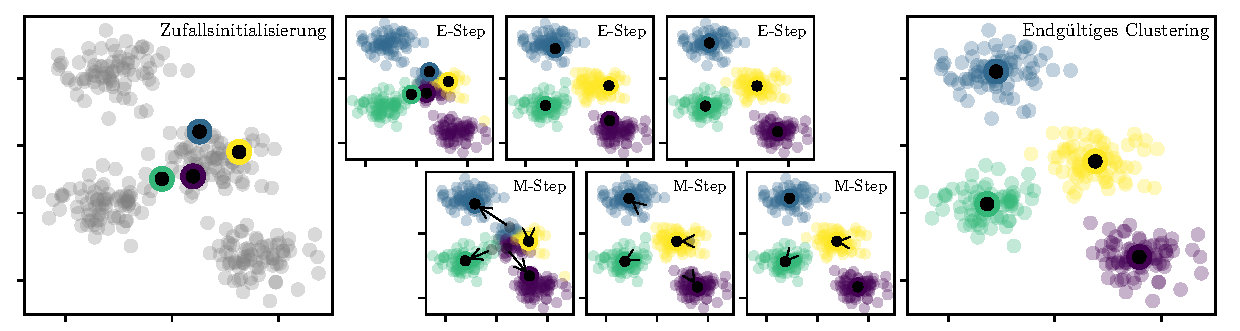
\includegraphics[width=\textwidth]{Bilder/expectation-maximization}
    \caption{Exemplarische Darstellung eines zweidimensionalen Clusterings mit Hilfe des EM-Algorithmus \cite{VanderPlas2016}}\label{fig:k-means}
\end{figure}


\subsection{simBEV}\label{chap:simbev_theo}

% TODO: probabilistischen Ansatz mathematisch erklären. @Tim wie wird die Wahrscheinlichkeit je ts konkret festgelegt?

Mit Hilfe des im Rahmen dieser Masterarbeit mitentwickelten Software Tools \simbev können die Fahrtprofile für eine beliebige Anzahl an Fahrzeugen verschiedener Fahrzeugklassen erstellt werden.
Weiterhin kann hierbei zwischen den in \autoref{tab:RegioStaR} aufgelisteten \Regiostar Raumtypen unterschieden werden, um das raumtypenspezifische Fahrverhalten abzubilden.
Zum Zeitpunkt der Erstellung der Fahrtprofile war es noch nicht möglich, einen längeren Zeitraum als eine Woche am Stück zu simulieren.

{
\renewcommand{\arraystretch}{1.2}% grßerer Zeilenabstand
\sisetup{range-phrase=~oder~}
\begin{table}[H]
	\begin{center}
		\caption{Regionalstatische Raumtypen (RegioStaR 7)}
		\begin{tabu} to \textwidth {X[1] X[2]}
			\hline
			Raumtyp Nummer & Regionalstatischer Raumtyp                                \\ \hline
			\num{71}       & Metropolen                                                \\
			\num{72}       & Regiopolen und Großstädte                                 \\
			\num{73}       & Mittelstädte, städtischer Raum einer Stadtregion          \\
			\num{74}       & Kleinstädtischer dörflicher Raum einer Stadtregion        \\
			\num{75}       & Zentrale Städte einer Ländlichen Region                   \\
			\num{76}       & Mittelstädte, städtischer Raum                            \\
			\num{77}       & Kleinstädtischer, dörflicher Raum einer Ländlichen Region \\ \hline
            \multicolumn{2}{l}{Quelle: \cite{BMVI2020}}
		\end{tabu}
		\label{tab:RegioStaR}
	\end{center}
	\vspace{-3mm}%Put here to reduce too much white space after your table
\end{table}
}

Die Fahrtprofile werden über einen probabilistischen Ansatz auf Grundlage der Befragung \gls{MID} \cite{ISGH2017} erstellt.
Dabei erhält jeder simulierte Zeitschritt eine Wahrscheinlichkeit für einen bestimmten Wegezweck eine Fahrt zu beginnen.
Löst ein Fahrzeug eine Fahrt aus, wird abhängig vom Wegezweck und Regionstyp der Fahrt, ebenfalls probabilistisch, eine Streckenlänge und eine anschließende Standzeit zugeteilt.
Der hierbei entstehende Verbrauch des Fahrzeuges muss anschließend gedeckt werden.
Ob am Zielort ein Ladevorgang stattfindet, hängt vom \gls{SOC} des Fahrzeuges und dem Vorhandensein eines Ladepunktes ab.
Ob ein Ladepunkt am Zielort zur Verfügung steht und welche Ladeleistung dieser aufweist, wird mit Hilfe der Wahrscheinlichkeiten aus \autoref{tab:WegezweckProbability2050} ermittelt.
Ladepunkte besitzen pauschal einen Wirkungsgrad von \SI{90}{\percent}. \cite{EliaGroup2020}
Die Bestimmung des Vorhandenseins eines Ladepunktes zu Hause und am Arbeitsplatz erfolgt je \gls{EPKW} einmalig und wird anschließend konstant gehalten.
Für alle anderen Wegezwecke, erfolgt die Bestimmung kontinuierlich.
Wurde dem Zielort ein Ladepunkt zugeordnet wird davon ausgegangen, dass der Fahrzeugnutzer einen Ladevorgang erst ab einem bestimmten \gls{SOC} einleitet, da dies einen zusätzlichen Aufwand für den Nutzer bedeutet.
Dabei wird angenommen, dass das Laden des Fahrzeuges am Wohnort und am Arbeitsplatz bereits ab einem \gls{SOC} von \SI{95}{\percent} stattfindet.
Im öffentlichen Raum bedeutet das Anfahren und der Anschluss an einen Ladepunkt einen größeren Aufwand für den Nutzer als im privaten Raum.
Deshalb wird angenommen, dass oberhalb eines \glspl{SOC} von \SI{80}{\percent} keine Ladevorgänge stattfinden.
Es gilt je niedriger der \gls{SOC}, desto wahrscheinlicher ist es, dass die öffentliche Ladeinfrastruktur genutzt wird.
Ab einem \gls{SOC} von \SI{50}{\percent} findet, wann immer möglich, eine Ladung des Fahrzeugs statt.
Zwischen den beiden Stützwerten erfolgt eine lineare Interpolation, welche in \autoref{fig:soc_charging_prob} visualisiert wurde.

\begin{figure}[H]
    \centering
    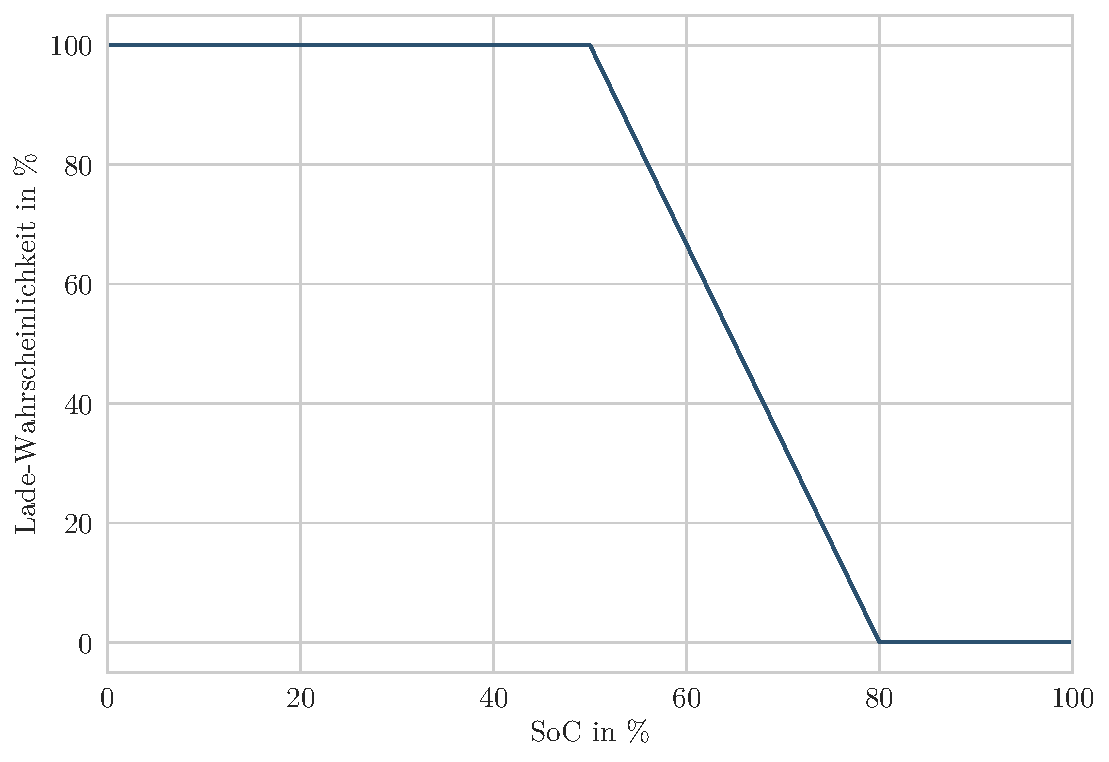
\includegraphics[width=\textwidth]{Bilder/soc_charging_prob}
    \caption{Abhängigkeit der Ladewahrscheinlichkeit vom SoC an öffentlichen Standorten}\label{fig:soc_charging_prob}
\end{figure}

Schnellladeinfrastruktur besitzt aufgrund des zusätzlichen Fahrt- und Zeitaufwandes eine geringe Attraktivität für den Nutzer.
Deshalb wird eine Schnellladung in dieser Simulation nur dann ausgelöst, wenn es wirklich nötig ist.
Sinkt der \gls{SOC} eines Fahrzeugs unter \SI{20}{\percent}, wird eine Schnellladestation angefahren und das Fahrzeug wird für \SI{15}{\Minuten} geladen.
Im Unterschied zu \glspl{BEV}, können \glspl{PHEV} auch mit einem \gls{SOC} von \SI{0}{\percent} ihre Fahrt mit Hilfe des Verbrennungsmotors fortsetzen.
Aus diesem Grund wird bei \glspl{PHEV} kein Schnellladevorgang ausgelöst.


\subsection{Räumliche Verteilung der Ladelast}

Die räumliche Verteilung der Ladelast innerhalb eines geographischen Gebietes kann starken Einfluss auf die Auswirkungen der Netzintegration von Elektrofahrzeugen haben.
So können beispielsweise regionale Konzentration von Ladepunkten einzelne Leitungen stark beanspruchen und den Netzausbaubedarf erhöhen.\medskip

Innerhalb dieser Arbeit erfolgt die Verteilung der Ladelast immer innerhalb des untersuchten Gebietes.
Ein Laden in anderen geographischen Gebieten, oder das Laden von \glqq Fremdfahrzeugen\grqq{} im untersuchten Gebiet kann nicht abgebildet werden.
Grundlage für die Ermittlung von möglichen Standorten bietet eine geoinformatische Auswertung der untersuchten geographischen Gebiete.
Das hierfür verwendete Software Tool, wurde unabhängig von dieser Arbeit am Reiner Lemoine Institut entwickelt und wurde noch nicht veröffentlicht.
An dieser Stelle soll die grundlegende Methodik für die Ermittlung von möglichen Standorten und deren Gewichtung für private und öffentliche Ladeinfrastruktur erläutert werden.
Eine genauere Beschreibung der Unterteilung in private und öffentliche Ladeinfrastruktur erfolgt in \autoref{chap:EMob_Szenarien} und die Ergebnisse der Verteilung werden in \autoref{chap:distribute_demand_ev} betrachtet.


\paragraph{Private Ladeinfrastruktur:}

Die private Ladeinfrastruktur beinhaltet alle Ladevorgänge, die an privater Ladeinfrastruktur am Eigenheim, in Wohnanlagen oder am Arbeitsplatz stattfinden.
Um mögliche Standorte für die Ladeinfrastruktur am Eigenheim oder in Wohnanlagen identifizieren zu können, werden die Anzahl an Wohneinheiten auf einem \SI{100 x 100}{\m} Raster aus dem Zensus 2011 \cite{StatistischesBundesamt2011} verwendet.
So wird jedem Raster mit mehr als einer Wohneinheit ein möglicher Anschlusspunkt für Ladeinfrastruktur zugeordnet und anhand der Gesamtanzahl von Wohneinheiten im Raster gewichtet.\medskip

Für private Ladeinfrastruktur am Arbeitsplatz werden die Klassifizierungen der Landflächen nach Nutzungsart nach der \gls{OSM} \cite{OpenStreetMapFoundation} verwendet.
Hierbei wird jeder Landfläche mit der Nutzungsart \glqq commercial\grqq , \glqq retail\grqq{} und \glqq industrial\grqq{} ein möglicher Anschlusspunkt für Ladeinfrastruktur zugeordnet.
Die Gewichtung erfolgt anhand der Fläche des Gebietes multipliziert mit einem Flächnutzungsfaktor.
Der Flächennutzungsfaktor liegt für \glqq commercial\grqq{} bei \num{3}, für \glqq retail\grqq{} bei \num{2} und für \glqq industrial\grqq{} bei \num{1}.


\paragraph{Öffentliche Ladeinfrastruktur:}

Die öffentliche Ladeinfrastruktur beinhaltet Ladeinfrastruktur, die nicht der privaten Ladeinfrastruktur zugeordnet werden kann.
Grundsätzlich lässt sich hierbei zwischen Normal- und Schnellladeinfrastruktur unterscheiden.
Für die Normalladeinfrastruktur werden allen \glspl{POI} aus der \gls{OSM} \cite{OpenStreetMapFoundation} in dem untersuchten Gebiet jeweils ein möglicher Anschlusspunkt für Ladeinfrastruktur zugeordnet.
Die Gewichtung der Anschlusspunkt erfolgt hierbei anhand der Gesamtanzahl an \glspl{POI} in der Nähe des Anschlusspunktes.\medskip

Für Schnellladeinfrastruktur werden jeder Tankstelle aus der \gls{OSM} \cite{OpenStreetMapFoundation} im untersuchten Gebiet jeweils ein Anschlusspunkt zugeordnet.
Eine Gewichtung findet in diesem Fall nicht statt.


\paragraph{Zuteilung der Ladevorgänge auf die Ladeinfrastruktur:}

Die Zuteilung der Ladevorgänge auf die Ladeinfrastruktur erfolgt mit Hilfe des Gewichtungsfaktors der verschiedenen Ladeinfrastrukturen.
Mit Hilfe des Zufallsmoduls des Open Source Tools \texttt{NumPy}, erfolgt eine zufällige und gewichtete Auswahl eines Anschlusspunktes je Ladevorgang.
Im Falle der privaten Ladeinfrastruktur wird für jedes Fahrzeug ein eigener Ladepunkt eingerichtet, wenn diese Ladevorgänge am Eigenheim, in Wohnanlagen oder am Arbeitsplatz aufweisen.
Diesem Ladepunkt werden alle Ladevorgänge des jeweiligen Fahrzeuges und \UCs zugeordnet.
Nachdem einem Anschlusspunkt ein Ladepunkt zugeordnet wurde, wird die Gewichtung des Anschlusspunktes leicht abgesenkt.
Für die öffentliche Ladeinfrastruktur erfolgt die Zuweisung dezidiert je Ladevorgang.
Je Ladevorgang wird untersucht, ob bereits ein passender Ladepunkt zur Verfügung steht.
Hierbei wird beachtet, ob in diesem Zeitraum der Ladepunkt durch ein anderes Fahrzeug besetzt ist und ob der Ladepunkt die entsprechende Ladeleistung zur Verfügung stellen kann.
Sollte kein passender Ladepunkt zur Verfügung stehen, wird analog zum Vorgehen bei der privaten Ladeinfrastruktur ein Ladepunkt zufällig und gewichtet ausgewählt und eingerichtet.


\subsection{eDisGo}\label{chap:edisgo_theo}

Das Open Source Tool \edisgo (\textbf{e}lectricity \textbf{Dis}tribution \textbf{G}rid \textbf{o}ptimization) stellt eine Toolbox zur Verfügung, um Verteilnetze auf Netzprobleme zu untersuchen.
Gleichzeitig können mit \edisgo Maßnahmen zur Behebung der Netzprobleme bewertet werden.
Dabei bilden synthetische Netztopologien, die mit Hilfe des Open Source Tools \dingo erzeugt wurden, die Grundlage für die Berechnungen mit \edisgodot.
\edisgo kann über GitHub \cite{edisgoGit2019} abgerufen werden und ist auf Read the Docs \cite{edisgoDocs2017} dokumentiert.
Innerhalb dieses Kapitels werden die wichtigsten Funktionalitäten \texttt{eDisGo}~ für die Durchführung der Berechnungen innerhalb dieser Masterarbeit dargestellt und erläutert.


\paragraph{Ermittlung von Netzproblemen:}\label{chap:grid_issues}

Die Überprüfung der einzelnen Netze auf Netzprobleme erfolgt in zwei Schritten.
Vorerst wird eine nichtlineare Lastflussberechnung durchgeführt, um anschließend die Einhaltung der Spannungsanforderungen und technischen Richtlinien bezüglich der Gerätebelastungen zu überprüfen.
Die Durchführung der Lastflussberechnung erfolgt mit Hilfe des Open Source Tools \texttt{PyPSA} \cite{Brown2020}.
In diesem Kapitel soll auf die theoretischen Grundlagen der Lastflussberechnung, den Umfang der Analyse und die Spannungsanforderungen und technischen Richtlinien bezüglich der Gerätebelastungen eingegangen werden.\medskip

Das Ziel der Lastflussberechnung ist es, das für jeden Netzknoten $i$ und etwaige Querleitwerte $j$ die folgende Gleichung erfüllt wird:

\begin{equation}
	S_i = P_i + j Q_i = V_i I_i^* = V_i \left(\sum_j Y_{ij} V_j \right)^*
	\label{eq:pf}
\end{equation}

\noindent Wobei:

\addvbuffer[12pt 12pt]{
	\begin{tabular}{>{$}r<{$}@{\ :\ }l}
		S_i 		& Scheinleistung am Netzknoten $i$ \\
		P_i	 		& Wirkleistung am Netzknoten $i$ \\
		Q_i			& Blindleistung am Netzknoten $i$ \\
		V_i			& Komplexe Spannung am Netzknoten, wobei $V_i = \left| V_i \right|e^{j \theta_i}$ \\
		I_i			& Stromstärke am Netzknoten \\
		Y_{ij}		& Admittanzmatrix am Netzknoten \\
	\end{tabular}
}

Der Winkel der komplexen Spannung ist relativ zum Potentialknoten.
Unter dem Potentialknoten wird ein Netzknoten verstanden, an welchem der Wirk- und Blindleistungsfluss frei eingestellt werden kann.
Mit Hilfe des Potentialknotens kann über einen iterativen Prozess die Konvergenz nach \autoref{eq:pf} des Systems erreicht werden.
Eine genau Beschreibung der Lastflussberechnung des Open Source Tools \texttt{PyPSA} kann auf Read the Docs \cite{Brown2020a} abgerufen werden.
Innerhalb dieser Masterarbeit wird als Potentialknoten die Sekundärseite des \gls{HS}-\gls{MS}-Umspannwerkes eines \gls{MS}-Netzes verwendet.
Alle weiteren Netzknoten werden mit gegebenen Wirk- und Blindleistungen modelliert. \cite{Schachler}\medskip

Die Lastflussanalyse der Netze berücksichtigt sowohl \gls{MS}- und \gls{NS}-Leitungen als auch die \gls{MS}-\gls{NS}-Umspannebene.
Gegenüber einer Aggregation der Erzeugung und des Bedarfs der einzelnen \gls{NS}-Netze an dem jeweiligen \gls{MS}-\gls{NS}-Umspannwerk bietet diese besonders tiefgehende Betrachtung die Möglichkeit, die Auswirkungen der teilweise hohen Ladeleistungen der Ladeinfrastruktur genauer zu betrachten und den Einfluss verschiedener Ladestrategien besser bestimmen zu können.
Da die Sekundärseite des \gls{HS}-\gls{MS}-Umspannwerkes als Potentialknoten modelliert wird, können an dieser keine Spannungsprobleme auftreten.
Jedoch entspricht die Scheinleistung des Potentialknotens der Leistung, die über das \gls{HS}-\gls{MS}-Umspannwerk geleitet wird.
Anhand dieses Wertes können zusätzlich Aussagen über die Überlastung des \gls{HS}-\gls{MS}-Umspannwerks getroffen werden.
Mit Hilfe der durch die Lastflussanalyse ermittelten Belastungen und Spannungsabweichungen an den Betriebsmitteln, können abschließend Überlastungen und Spannungsprobleme festgestellt werden.
Eine Übersicht über den Umfang der Lastflussanalyse findet sich in {\color{red} TODO}. \cite{Schachler}

{\color{red} TODO}


\paragraph{Ermittlung des Abregelungsbedarfs für die Auflösung von Netzüberlastungen:}

Die Ermittlung des Abregelungsbedarfs für die Auflösung von Netzüberlastungen erfolgt in einem iterativen Prozess.
Vorerst werden etwaige Netzprobleme und die entsprechenden Zeitschritten in denen die Netzprobleme auftreten mit Hilfe der zuvor beschriebenen Lastflussanalyse ermittelt.
Anschließend wird die Last bzw. die Einspeisung in Schritten von \SI{10}{\percent} innerhalb der ermittelten Zeitschritte gekürzt.
Die beiden Schritte werden so lange wiederholt, bis keine Netzprobleme mehr auftreten.\medskip

Bei der Lösung der Netzprobleme werden vorerst Überlastungen gelöst und erst anschließend Spannungsprobleme.
Weiterhin werden Probleme in der \gls{NS}-Ebene gelöst, bevor Probleme in der \gls{MS}-\gls{NS}-Umspannebene und abschließend in der \gls{MS}-Ebene gelöst werden.
Durch die Lösung von Netzproblemen auf tieferen Spannungsebenen können unter Umständen bereits Netzprobleme in darüber liegenden Spannungsebenen gelöst oder entspannst werden.
Weiterhin werden Netzprobleme innerhalb der \gls{NS}- bzw. \gls{MS}-Ebene anhand ihrer Entfernung zur übergeordneten Umspannebene priorisiert.
So kann auch hier die Lösung von weiter entfernten Netzproblemen bereits vorgeschaltete Netzprobleme auflösen oder entspannen.
Für jeden Zeitschritt, in dem Überlastungs- oder Spannungsprobleme an einem Netzknoten auftreten, wird geprüft, ob die Netzprobleme durch hohe Nachfrage oder hohe Einspeisung entstehen.
Anhand dieser Information wird entscheiden, ob Last oder Einspeisung abgeregelt werden soll.
Die gesamte notwendige Abregelung für das \gls{MS}-Netz erfolgt abschließend über die Summierung aller nötigen Abregelungen von Last und Erzeugung am \gls{MS}-Netzanschlusspunkt.
In {\color{red} TODO} findet sich eine Darstellung des Vorgehens.

{\color{red} TODO}


\subsection{Untersuchte Ladestrategien}

Innerhalb dieser Arbeit werden zwei präventive Ladestrategien und eine kurative Ladestrategie untersucht.
Das Ziel der Ladestrategien ist es, ein möglichst netzfreundliches Verhalten aufzuweisen, ohne den Nutzen des Fahrzeuges einzuschränken.
Deshalb gilt als Randbedingung aller Ladestrategien, dass der Ladebedarf jedes Ladevorgangs zu \SI{100}{\percent} gedeckt werden muss.
Dies bedeutet, dass Ladevorgänge nur dann flexibilisiert werden können, wenn innerhalb der Standzeit eine Vollladung möglich ist.
Weiterhin können nur private Ladevorgänge flexibilisiert werden, da bei öffentlichen Ladevorgängen die Erfüllung der Dienstleistung im Vordergrund steht.\medskip

Um die drei Ladestrategien miteinander vergleichen zu können, wird zusätzlich ein vollkommen ungesteuertes Laden der Fahrzeuge untersucht, welches als Vergleichspunkt verwendet wird.
Auf diese Weise soll untersucht werden, inwieweit eine kurative Ladestrategie gegenüber präventiven Ladestrategien Vorteile aufweist.
Dies ist deshalb von Bedeutung, da für kurative Eingriffe zusätzliche Technik eingesetzt und die  Betriebsführung dieser abgebildet werden muss, wodurch die Kosten einer kurative Ladestrategie deutlich über den Kosten einer präventiven Ladestrategie liegen.


\paragraph{Gruppiertes Laden:}

Das Ziel des gruppierten Ladens ist es, die Netzbelastung durch die Senkung der Gleichzeitigkeit der Ladevorgänge zu reduzieren.
Hierfür werden die einzelnen Ladepunkte in zwei Gruppen eingeteilt.
Beiden Gruppen werden alternierend 15-minütige Ladezeitfenster zugewiesen, in denen bei voller Ladeleistung der Ladebedarf gedeckt wird.
Es wird darauf geachtet, dass die Zuweisung der Gruppen nicht nur innerhalb eines Netzgebietes ausgeglichen erfolgt, sondern detailliert bis in die einzelnen Stränge der \gls{NS}-Ebene.
Innerhalb eines \gls{NS}-Stranges wird weiterhin darauf geachtet, dass auch die einzelnen Leistungsklassen der Ladeinfrastruktur gleichmäßig auf die Gruppen verteilt werden.
In {\color{red} TODO} findet sich eine beispielhafte Einteilung von Ladepunkten auf die zwei Gruppen innerhalb eines \gls{NS}-Stranges.


{\color{red} TODO: Veranschaulichung}


\paragraph{Reduziertes Laden:}

Im Gegensatz zum gruppierten Laden soll beim reduzierten Laden die Senkung der Netzbelastung durch die Reduzierung der Ladeleistung der einzelnen Ladevorgänge erreicht werden.
Hierbei wird durch eine Absenkung der Ladeleistung möglichst die gesamte Standzeit des Fahrzeuges für den Ladevorgang ausgenutzt.
Die Flexibilität dieser Ladestrategie wird durch eine Mindestladeleistung von \SI{10}{\percent} der Nennleistung des angefahrenen Ladepunktes technisch begrenzt.

% TODO: Quelle Konferenzpaper Birgit?


\paragraph{Residuallast-Laden:}

Bei dem Residuallast-Laden handelt es sich um eine kurative Ladestrategie.
Der Ladevorgang eines Fahrzeuges findet hierbei immer innerhalb der Zeitpunkte der Standzeit statt, welche die geringste Residuallast aufweisen, wodurch eine Glättung der Residuallast erreicht werden soll.
Die Zuweisung findet auf Viertelstundenbasis statt und die Ladevorgänge finden immer bei voller Ladeleistung statt.
Das Ziel der Optimierung kann nach \autoref{eq:residual} so formuliert werden, dass eine Minimierung der \gls{MQA} der Residuallast vom Mittelwert der Residuallast angestrebt wird.

\begin{equation}
	\text{MQA} = \frac{1}{n} \sum_i^n \left( P_{\text{R}_i} - \overline{P}_{\text{R}} \right)^2 \stackrel{!}{=} \text{min}
	\label{eq:residual}
\end{equation}

\noindent Wobei:

\addvbuffer[12pt 12pt]{
	\begin{tabular}{>{$}r<{$}@{\ :\ }l}
		P_{\text{R}_i}				& Residuallast zum Zeitschritt $i$  \\
		\overline{P}_{\text{R}}		& Mittelwert der Residuallast 		\\
		n							& Anzahl an Zeitschritten			\\
		i							& Index des Zeitschrittes 			\\
	\end{tabular}
}

Durch die Abhängigkeit der Residuallast von den einzelnen Ladevorgängen sind auch die Ergebnisse der Optimierung der einzelnen Ladevorgänge voneinander Abhängig.
Hierdurch entsteht ein komplexes Optimierungsproblem.
Um die Rechenzeit in einem akzeptablen Maß zu halten, wird eine Näherung an eine optimale Lösung angestrebt.
So wird für jeden Ladevorgang ermittelt, wie viel überschüssige Standzeit zur Flexibilisierung der Ladevorgänge zur Verfügung steht.
Die Ladevorgänge werden anschließend in Abhängigkeit dieses Kriteriums in aufsteigender Reihenfolge sortiert und einzeln optimiert.
Auf diese Weise werden Ladevorgänge mit einem geringen Flexibilitätsband vorrangig behandelt und eine möglichst optimale Lösung bei einem geringen Rechenaufwand erreicht.

% TODO: kurativ vs aktiv. Was ist das bessere Wort?
